\documentclass[11pt,a4paper]{article}
\usepackage{fontspec}
\setmainfont{Source Serif 4}[Path=/home/claude/ref/fonts/, UprightFont=SourceSerif4-Regular.ttf, BoldFont=SourceSerif4-Semibold.ttf, ItalicFont=SourceSerif4-It.ttf]
\setmonofont{IBM Plex Mono}[Path=/home/claude/ref/fonts/, UprightFont=IBMPlexMono-Regular.ttf, BoldFont=IBMPlexMono-Medium.ttf, Scale=0.88]
\usepackage[a4paper,margin=2.4cm]{geometry}
\usepackage{amsmath}
\usepackage{graphicx,booktabs,float,caption,array,xcolor,longtable}
\usepackage{xurl}
\usepackage[hidelinks]{hyperref}
\usepackage[round]{natbib}
\usepackage{setspace}
\setstretch{1.08}
\renewcommand{\topfraction}{0.9}
\renewcommand{\bottomfraction}{0.8}
\renewcommand{\textfraction}{0.1}
\renewcommand{\floatpagefraction}{0.75}
\setlength{\parindent}{0pt}
\setlength{\parskip}{0.55em}
\captionsetup{font=small,labelfont=bf}
\setlength{\bibsep}{3pt}
\urlstyle{same}
\hypersetup{pdftitle={Lost Money: Roman Coin Loss across England by District and Reece Period},pdfauthor={Dr Tristan Hotham}}

\begin{document}
\begin{center}
{\Large\bfseries Lost Money: Roman Coin Loss across England by District and Reece Period, from the Portable Antiquities Scheme\par}
\vspace{1.2em}
{\large Dr Tristan Hotham\par}
\vspace{0.3em}
{\small Independent researcher\\
ORCID: 0000-0003-4931-9349\\
DOI: https://doi.org/10.5281/zenodo.24115196\par}
\vspace{0.8em}
2026
\end{center}

\begin{quote}
\small
\begin{center}\textbf{Abstract}\end{center}
Roman coins are closely dated and common among finds reported by the public in England. I use facet counts from the public search of the Portable Antiquities Scheme (PAS) to build a complete district-level table for England: 275,206 Roman coin records, 188,831 of them assigned to one of Reece's 21 issue periods, set against 1,062,032 records of all periods that measure how intensively each of 296 districts is detected and recorded. The English profile reproduces the classic British site-find curve: loss per year is highest in AD 330 to 348 (4.8 times a flat rate), then AD 364 to 378 and AD 260 to 275, and 82\% of dated coins are later than AD 260. I then test, with a plan written before any district shares were computed, whether the share of late coins (AD 364 to 402) rises smoothly towards the south and east and the share of early coins (before AD 222) towards the north and west. Neither gradient is supported: per 100 km east the odds ratio for the late share is 0.94 (95\% CI 0.83 to 1.06), and per 100 km north 0.98 (0.89 to 1.08), and all but one of 20 planned checks agree. In exploratory analysis the variation takes the form of a step: in the North East and North West, 4.3\% of dated coins are late against 15.9\% elsewhere, and 58\% are early against 15\%. The contrast looks like a frontier zone set against the rest of England, not a continuous tilt.

\textbf{Keywords:} Roman Britain; coinage; site finds; Reece periods; Portable Antiquities Scheme; metal detecting; regional variation; England
\end{quote}

\section{Introduction}\label{sec:intro}
Coins are the most closely dated objects that the inhabitants of Roman Britain lost in large numbers. Each carries the name of an emperor, and the issues of each reign reached the province in quantities that changed sharply from one decade to the next. Since \citet{reece1972} compared the coins from fourteen excavated sites, numismatists have used the share of a site's coins that falls in each of a set of fixed issue periods to describe when the site was busy, how it compares with the average British site, and how it differed from sites on the Continent \citep{casey1986,reece1987,reece1995}. The method rests on a simple observation: coins that were lost and never recovered are a sample of the coins that were in use, and if every site drew from the same pool, differences in the proportions of coins from each period tell us about the sites rather than about the supply.

The Portable Antiquities Scheme (PAS), which since 1997 has recorded archaeological objects found by members of the public in England and Wales, has transformed the quantity of evidence available for this kind of analysis \citep{bland2005,bland2017,lewis2016}. Roman coins are its largest single class of record. \citet{walton2012} used the first decade of PAS coin data to rethink Roman Britain region by region, \citet{brindle2014} used PAS Roman material to study rural settlement, and \citet{henry2024} has combined PAS records with excavated and museum assemblages into a corpus of 490,154 site-find coins, most of them mapped by parish. Each of these studies has had to face the same problem: the PAS records what people find and choose to report, and the distribution of finds owes as much to land use, access, the habits of detectorists and the capacity of Finds Liaison Officers as to the past \citep{robbins2012,robbins2013,cooper2016}.

This paper takes a deliberately simple route through that problem. Instead of the individual records, I use the counts that the PAS public search returns when its results are grouped by district and by Reece period, for every English ceremonial county. Those counts are complete for England at district level, the finest level at which PAS findspots are public, and they include a denominator that most coin studies lack: the number of records of every period and type found in each district. The share of all records that are Roman coins, and the share of a district's dated coins that belong to each period, are both measured against that background of recording.

I ask three questions. First, does the English PAS profile across Reece's periods reproduce the shape that \citet{reece1995} described for British sites? It does, closely. Second, does the share of late coins rise smoothly towards the south and east, and the share of early coins towards the north and west, as a reading of the literature on late Roman Britain might suggest \citep{esmondecleary1989,walton2012,walton2016}? I wrote this test down before computing any district shares, and it fails: neither gradient is distinguishable from zero, under the planned model or in all but one of 20 variants of it. Third, what form does regional variation take instead? In exploratory analysis it appears as a step rather than a slope: districts in the North East and North West, the frontier zone of the province, have about a quarter of the late share and four times the early share of districts elsewhere, while the South West, the furthest west of all English regions, has the highest late share.

The contribution is threefold. The paper provides a complete, reproducible district-by-period table of PAS Roman coin records for England, with the all-finds denominator, built from the public search alone. It reports a pre-specified test of a widely held but rarely formalised idea, with a null result that I think is informative. And it shows, with every number traceable to a single results file, how the Reece method can be run at the scale of the whole country while being explicit about what recording bias it does and does not remove.

Section~\ref{sec:lit} reviews the coin-loss literature, regional work on Roman Britain and studies of PAS bias. Section~\ref{sec:data} describes the data and Section~\ref{sec:design} the design. Section~\ref{sec:results} reports the results and Section~\ref{sec:robust} the robustness checks. Section~\ref{sec:disc} discusses the findings and their limits.

\section{Background and literature}\label{sec:lit}
\subsection{Coin loss and the Reece method}
Site finds are coins that were lost and never recovered, as distinct from hoards deliberately put away, and archaeologists and numismatists have increasingly argued that coins should be studied as archaeological material in their own right, for what their contexts say about use as well as about issue \citep{casey1986,kemmers2011}. \citet{reece1972} showed that, when the coins from fourteen British sites were divided into a set of fixed periods, the sites shared a common pattern that differed from Continental sites. He later formalised the method into 21 periods from the pre-Claudian coinage to AD 402, and used it to compare 140 British sites \citep{reece1991} and then to summarise the British pattern as a whole \citep{reece1995}. The British curve has low coin loss from the conquest to about AD 260, high loss from about 260 to 294, a dip from 294 to 330, a major peak from 330 to 348 and generally high loss for the rest of the fourth century \citep{reece1995}. \citet{reece1995} notes that John Casey, working on coins from military sites, had independently reached similar conclusions; \citet{casey1986} is his introduction to coins for archaeologists and historians.

The method has been tested and extended. \citet{lockyear2000} compared the techniques used to analyse British site-find assemblages, and \citet{ryan1988} analysed fourth-century coin finds from Roman Britain by computer. \citet{davies1991} used reported finds from Norfolk to describe coin use across a single civitas, an early demonstration that public finds could be read in the same way as excavated assemblages. The per-mille profile and its comparison with a British mean remain the standard way to write a coin report \citep{henry2024}.

\subsection{Regional variation in Roman Britain}
A long tradition divides Roman Britain into a civil south and east and a military north and west, a division that echoes the Highland and Lowland zones of \citet{fox1932} and runs through modern accounts of the province \citep{millett1990,mattingly2006}. Coin evidence has been read in the same way. In Henry's corpus, early coin loss is strongest at military sites, and later fourth-century loss is strongest in the south, parts of the Midlands and East Anglia, while the east coast from Norfolk to Essex regularly falls in the lower quartile \citep{henry2024}. \citet{walton2016} map the silver siliquae of AD 388 to 402 as concentrated in southern and eastern lowland Britain and extending into parts of Yorkshire, with finds sparse in the south-west, Wales, the west Midlands, and the north-west and north-east. The rural economy volume of the Roman Rural Settlement Project discusses coins and markets in the countryside \citep{brindle2017}.

\citet{walton2012} analysed the PAS coin records, then about 220,000 coins, alongside coins from excavated sites, to ask when, where, by whom and for what purpose coinage was used, and considered regionality explicitly. \citet{moorhead2013} illustrated the history of Roman coinage in Britain entirely with PAS finds. \citet{moorhead2014} and \citet{walton2016} reviewed the numismatic evidence for the end of Roman Britain, using hoards and site finds to ask how far coin use continued after the last new issues arrived around AD 402. \citet{bland2018} studied coin hoards and hoarding across the province. \citet{collins2012} examined the frontier in the fourth and fifth centuries, and \citet{gerrard2013} the archaeology of the end of Roman rule more broadly.

The most comprehensive recent work is \citet{henry2024}, who mapped per-mille values in grouped phases for 1,421 parishes with at least 25 coins. Early coin loss is strongest at military sites in Wales, on Hadrian's Wall and in the Pennines, and the later fourth century is strongest in a band through Hampshire, Wiltshire, Gloucestershire, Oxfordshire, the East Midlands and parts of East Anglia, with some coastal areas of the east and south in the lower quartile. Henry's maps suggest that the late Roman pattern is not a simple east to west tilt, and that is the possibility this paper tests formally.

\subsection{The Portable Antiquities Scheme as evidence}
The PAS is a voluntary scheme, run by the British Museum with Amgueddfa Cymru in Wales, that records finds made by the public, mostly by metal detecting \citep{bland2005,bland2017,lewis2016}. Its database has been used for regional syntheses of Roman Britain \citep{brindle2013,brindle2014}, for Anglo-Saxon and Viking-age economies \citep{richards2009} and for long-term landscape studies \citep{cooper2016}. Every such study confronts recording bias. \citet{robbins2012} identified seven stages at which bias can enter the PAS record, from deposition to recording, and \citet{robbins2013} showed with case studies how they shape distributions at different scales. Ploughed land is detected more than pasture or woodland; access and landowner permission vary; some areas have more active detectorists or more recording staff; and some kinds of object are more likely to be recognised and reported than others. \citet{bevan2012} proposed comparing artefact distributions with the distribution of all recorded finds, so that a pattern is judged against where anyone has looked. This paper follows that logic by using all PAS records of every period in a district as the denominator for Roman coins.

\subsection{Expectations}
From this literature I wrote down four expectations before computing any district shares. The English PAS profile should reproduce the British site-find curve (H1). The share of late coins should rise towards the east and fall towards the north (H2). The share of early coins should do the opposite (H3). And Roman coins should make up a larger share of all finds in the south and east (H4). H2 to H4 are written as smooth gradients, because the simplest version of the civil and military contrast is a tilt across the country, and because a gradient can be tested against a clear null.

\section{Data}\label{sec:data}
\subsection{PAS facet counts}
The data are facet counts from the public search of the PAS database (\url{https://finds.org.uk}), retrieved through its application programming interface in 2026. For each of England's 47 ceremonial counties as recorded by the PAS (the City of London is recorded within Greater London), five kinds of query were made: all records of any period or type, by district; Roman coin records, by district; Roman coin records by Reece period for the county; Roman coin records of each Reece period, by district; and the 50 commonest rulers on Roman coin records in the county. National facets were retrieved for Reece periods, rulers and counties. Altogether there are 1,317 queries, with no failed requests. Counts are of records, not coins: a PAS record can describe more than one coin, and some hoards are recorded coin by coin. Table~\ref{tab:data} summarises the data.

\begin{table}[tbp]\centering\small\caption{The data: PAS facet counts for England, retrieved 2026.}\label{tab:data}\begin{tabular}{lr}\toprule Item & Number\\\midrule
Ceremonial counties queried & 47\\
Districts (ONS 2023) & 296\\
District names in the PAS data matched to ONS names & 296 of 296\\
All PAS records, county totals & 1,062,193\\
\quad with a district & 1,062,032\\
Roman coin records & 275,206\\
\quad with a Reece period 1 to 21 & 188,831\\
\quad Reece periods 22 to 24 (excluded) & 34\\
Roman coin records per 1,000 records & 259.1\\
Districts with at least 20 dated coin records & 173\\
Districts with at least 100 dated coin records & 127\\
Districts with no Roman coin record & 22\\
PAS national Reece facet, periods 1 to 21 (incl.\ Wales) & 239,978\\\bottomrule\end{tabular}\end{table}

The API returns at most 50 values for any facet. The longest district list has 33 names (Greater London), so the district counts are complete. The ruler lists are the top 50 in each county and are used only descriptively.

\subsection{Districts and coverage}
Findspots are public only to district level. All 296 district names in the data match the names of the Office for National Statistics' Local Authority Districts (December 2023) exactly, and every one of England's 296 districts appears; no name had to be merged into a successor authority, because the PAS has already moved records to the districts created in 2019 and 2023 (for example Cumberland, Westmorland and Furness, and North Yorkshire). Eleven district names appear under more than one ceremonial county, usually because a record's county and district disagree (57 records in all); counts are summed by district, which counts each record once, and the district is assigned to the county holding most of its records. District sums fall 161 records short of the county totals, the records with no district.

The data cover England only. Welsh finds appear in the national county facet but under the Welsh principal areas, not the ceremonial counties used for the district queries, so they were not retrieved. All results and labels are therefore for England.

Boundaries are the ONS Local Authority Districts (December 2023) Boundaries UK BSC, with districts assigned to the nine English regions by the region containing a point inside each district. Coordinates are the easting and northing of that point on the British National Grid.

\subsection{Reece periods}
The PAS assigns Roman coins to Reece periods 1 to 21 and to three later periods (22 to 24) for fifth- and sixth-century coins. Their dates are taken from the Nomisma.org concepts \texttt{reece1} to \texttt{reece24}, which match the PAS list. Periods 22 to 24 hold only 34 English records and are excluded from the analysis. Of all Roman coin records, 68.6\% have a Reece period from 1 to 21; the rest are too worn or too fragmentary to place.

\section{Research design}\label{sec:design}
\subsection{Analysis plan}
The analysis plan was written in the study's notes before any district shares, gradients or models were computed, and is pre-specified in a written plan included in the data archive. At that point the structure of the data had been checked, which meant that the national Reece-period totals and county totals had been seen. H1 is therefore a replication check rather than a blind test. Nothing regional had been computed. Everything not in the plan is labelled exploratory.

\subsection{Measures}
For each district $i$ let $N_i$ be all PAS records, $C_i$ Roman coin records, $D_i$ coin records with a Reece period from 1 to 21, and $D_{ip}$ coin records in period $p$. The per-mille value of period $p$ is $1000 D_{ip}/D_i$; the per-year value divides it by the length of the period in years (period 1, which has no start date, has no per-year value). The late share is $L_i/D_i$ with $L_i = D_{i,19}+D_{i,20}+D_{i,21}$ (AD 364 to 402), the early share $E_i/D_i$ with $E_i = \sum_{p=1}^{10} D_{ip}$ (to AD 222), and the coin share $C_i/N_i$, reported as Roman coin records per 1,000 records.

\subsection{Models}
H2 to H4 are tested with binomial generalised linear models of a share on easting and northing (in units of 100 km):
\begin{equation}
\operatorname{logit} \Pr(\text{coin is late} \mid i) = \alpha + \beta_E\, \mathrm{east}_i + \beta_N\, \mathrm{north}_i,
\end{equation}
fitted to the counts $L_i$ out of $D_i$ for districts with $D_i \ge 20$ (N = 173), and likewise for $E_i$ out of $D_i$ and for $C_i$ out of $N_i$ (all 296 districts). This is the grouped-data form of the fractional logit model \citep{papke1996}. The counts are strongly overdispersed (Pearson dispersion 25.5 for the late share), so inference uses standard errors clustered by ceremonial county \citep{cameron2015}, which allow for both overdispersion and correlation between neighbouring districts in the same county. Results are reported as odds ratios per 100 km with 95\% confidence intervals. The hypothesis is supported if $\exp(\beta_E) > 1$ and $\exp(\beta_N) < 1$ for H2 and H4, and the reverse for H3, with intervals excluding 1. Models were fitted with statsmodels \citep{seabold2010}.

\subsection{Robustness and falsification}
The plan listed ten checks: minimum dated coins of 0, 50 and 100; weighted least squares on the empirical logit; standard errors clustered by region; leaving out each of the nine regions; dropping the ten districts with most coin records (large sites and hoards recorded coin by coin); dropping districts where one period holds more than 40\% of dated coins (another sign of hoards); two other definitions of late (after AD 378; after AD 330); adding the log of all records per square kilometre as a control for detecting intensity; a negative binomial count model with an offset for dated coins; and a spatial permutation test in which shares are shuffled across district locations 999 times.

\subsection{Threats to inference}
The design is descriptive. The denominator removes differences in how much is found and recorded in each district, but not differences in what is found within that total. Late Roman bronze coins are small and may be under-recovered or under-reported in some places more than others; ploughing brings different layers to the surface; and some districts contain a few large and productive sites that dominate their totals. The share models address the first issue only in part. Hoards recorded coin by coin can swamp a district's profile, which the checks address by dropping districts with very large or very concentrated assemblages. Districts are large and uneven units, and a gradient measured between them can hide variation within them.

\section{Results}\label{sec:results}
\subsection{The English profile}
Table~\ref{tab:profile} and Figure~\ref{fig:profile} give the English profile. The pattern is Reece's. Coin loss is low and fairly even from the conquest to AD 260, with per-year values below 1.2 per 1,000 in every period. It jumps in AD 260 to 275 (8.9 per 1,000 per year), the period of the Gallic emperors and of Claudius II, falls back through the Tetrarchy, and peaks in AD 330 to 348 under Constantine I and his sons (13.2), 4.8 times the flat rate of 2.77 that would apply if coins had been lost at the same pace in every year from AD 41 to 402. The Valentinianic period, AD 364 to 378, is the second highest (9.6). AD 378 to 388 holds only 6.2 per mille, 21 times less per year than AD 330 to 348, before a modest recovery in the last period. Coins later than AD 260 make up 82.4\% of all dated coins. H1 is supported, with the caveat that the national totals had been seen before the plan was written.

\begin{figure}[tbp]\centering
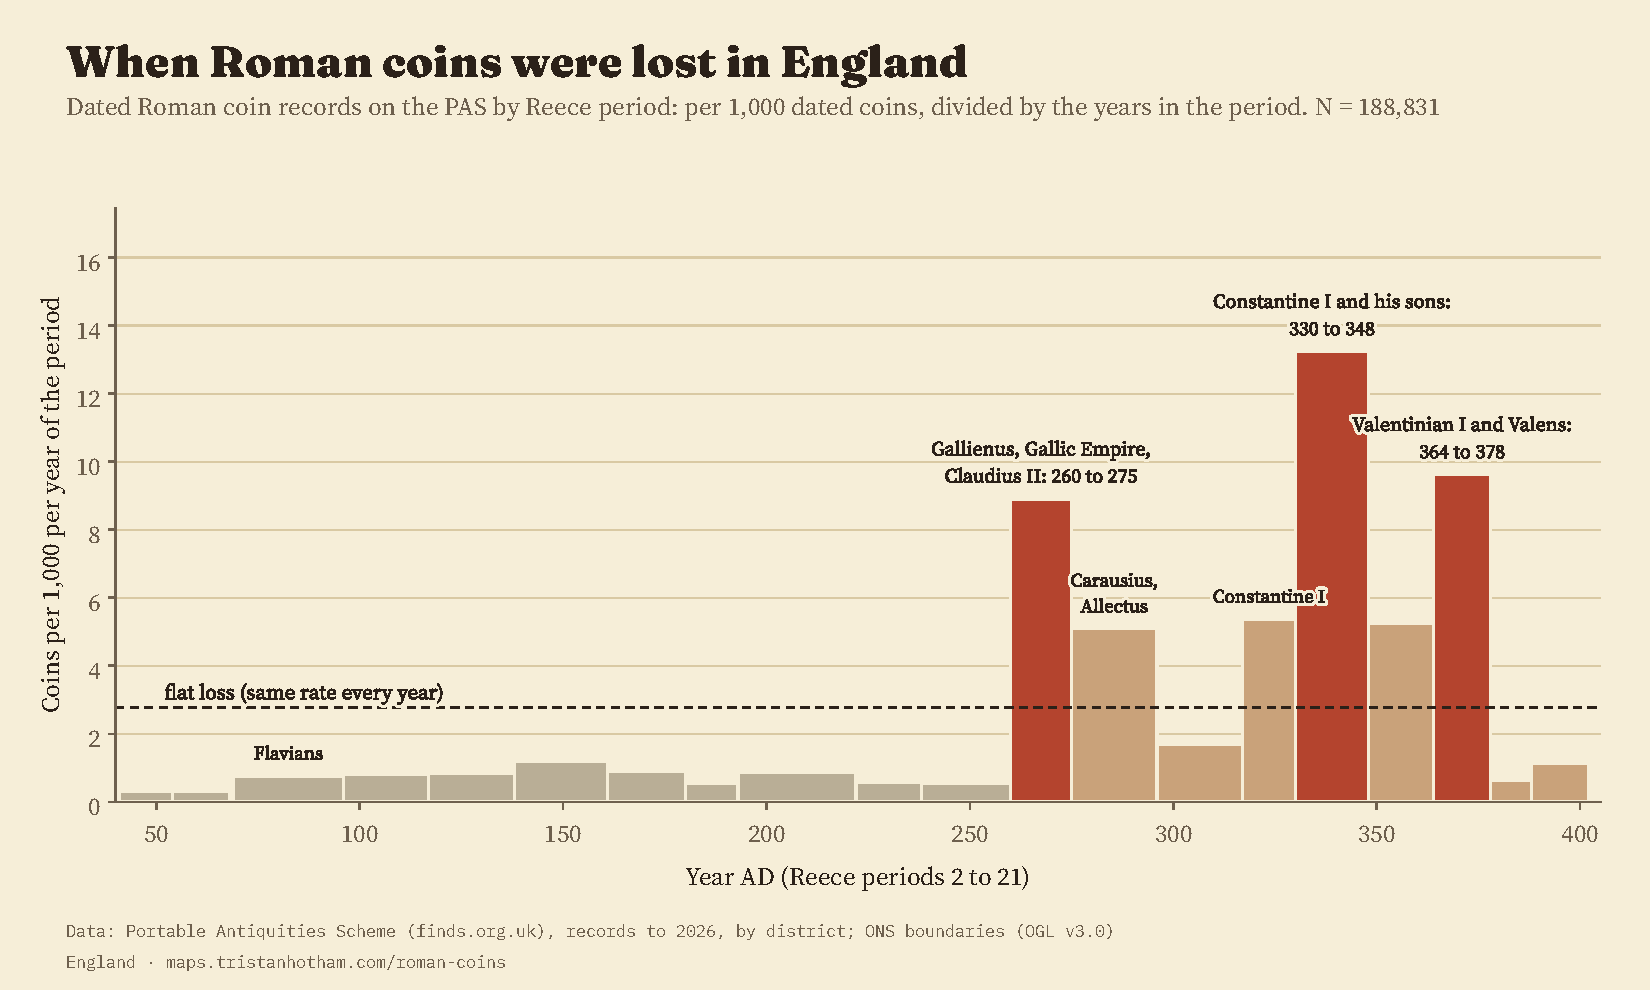
\includegraphics[width=\textwidth]{f_profile.pdf}
\caption{Roman coin loss per year in England by Reece period: per 1,000 dated PAS coin records, divided by the number of years in the period. N = 188,831. The dashed line is the value if coin loss had been even from AD 41 to 402.}\label{fig:profile}
\end{figure}

\begin{table}[tbp]\centering\footnotesize\caption{England's Roman coin profile by Reece period: dated PAS coin records, per mille and per mille per year. N = 188,831.}\label{tab:profile}\begin{tabular}{rllrrr}\toprule Period & Years AD & Main issuers & Records & Per mille & Per year\\\midrule
1 & to 41 & Republic and Iron Age, to AD 41 & 2,902 & 15.4 & \\
2 & 41 to 54 & Claudius & 778 & 4.1 & 0.32\\
3 & 54 to 68 & Nero & 776 & 4.1 & 0.29\\
4 & 69 to 96 & Vespasian, Titus, Domitian & 3,885 & 20.6 & 0.76\\
5 & 96 to 117 & Nerva, Trajan & 3,252 & 17.2 & 0.82\\
6 & 117 to 138 & Hadrian & 3,287 & 17.4 & 0.83\\
7 & 138 to 161 & Antoninus Pius & 5,164 & 27.3 & 1.19\\
8 & 161 to 180 & Marcus Aurelius & 3,220 & 17.1 & 0.90\\
9 & 180 to 193 & Commodus & 1,352 & 7.2 & 0.55\\
10 & 193 to 222 & Severus to Elagabalus & 4,754 & 25.2 & 0.87\\
11 & 222 to 238 & Severus Alexander, Maximinus & 1,726 & 9.1 & 0.57\\
12 & 238 to 260 & Gordian III to Valerian & 2,191 & 11.6 & 0.53\\
13 & 260 to 275 & Gallienus, Gallic Empire, Claudius II, Aurelian & 25,190 & 133.4 & 8.89\\
14 & 275 to 296 & Probus, Carausius, Allectus & 20,181 & 106.9 & 5.09\\
15 & 296 to 317 & The Tetrarchy & 6,648 & 35.2 & 1.68\\
16 & 317 to 330 & Constantine I & 13,191 & 69.9 & 5.37\\
17 & 330 to 348 & Constantine I and his sons & 44,960 & 238.1 & 13.23\\
18 & 348 to 364 & Constantius II, Magnentius, Julian & 15,849 & 83.9 & 5.25\\
19 & 364 to 378 & Valentinian I and Valens & 25,408 & 134.6 & 9.61\\
20 & 378 to 388 & Gratian, Theodosius, Magnus Maximus & 1,165 & 6.2 & 0.62\\
21 & 388 to 402 & Theodosius I, Arcadius, Honorius & 2,952 & 15.6 & 1.12\\
\bottomrule\end{tabular}\end{table}

\subsection{Planned tests of gradients}
Table~\ref{tab:main} gives the planned models. None of the six gradient coefficients has the predicted sign with an interval that excludes 1. The late share falls very slightly towards the east and the north, and both intervals include 1. The early share rises slightly towards the north (an odds ratio of 1.16, interval 0.93 to 1.43) and falls slightly towards the east (0.85, 0.65 to 1.12), the predicted signs, but both intervals include 1. The share of all records that are Roman coins falls towards the north (0.89, 0.78 to 1.03) but does not rise towards the east. H2, H3 and H4 are not supported. Spatial permutation gives the same verdict: the share of 999 shuffles with an easting coefficient at least as large as the observed one is 0.35 for the late share, 0.15 for the early share and 0.66 for the coin share.

\begin{table}[tbp]\centering\footnotesize\caption{Planned tests: binomial GLM odds ratios per 100 km east and north, 95\% CI, standard errors clustered by ceremonial county. H2 and H3: districts with at least 20 dated coin records. Dispersion is the Pearson statistic over residual degrees of freedom of the unclustered model.}\label{tab:main}\begin{tabular}{lrrrrrrr}\toprule Outcome & East OR [95\% CI] & $p$ & North OR [95\% CI] & $p$ & N & Clusters & Disp.\\\midrule
H2: late share, AD 364 to 402 & 0.94 [0.83, 1.06] & 0.320 & 0.98 [0.89, 1.08] & 0.660 & 173 & 46 & 25.5\\
H3: early share, to AD 222 & 0.85 [0.65, 1.12] & 0.241 & 1.16 [0.93, 1.43] & 0.191 & 173 & 46 & 91.9\\
H4: Roman coins of all records & 1.04 [0.85, 1.27] & 0.708 & 0.89 [0.78, 1.03] & 0.124 & 296 & 47 & 260.6\\
\bottomrule\end{tabular}\end{table}

\subsection{Exploratory: a step rather than a slope}
The absence of a gradient is not an absence of variation. Figure~\ref{fig:regions} shows the early and late shares by region and Table~\ref{tab:regions} in the appendix the full figures. In the North East and North West, 57.9\% of dated coins are early and 4.3\% late; in the other seven regions together, 14.7\% and 15.9\%. The West Midlands sits in between (26.7\% early, 9.6\% late). The South West, which lies as far west as the North West, has the highest late share of any region (17.2\%) and the lowest early share. A Wald test that all nine regions share one late share rejects strongly ($\chi^2$ = 201, 8 df). In a model with a single indicator for the two northern regions, the odds of a dated coin being late are 0.23 times those elsewhere (95\% CI 0.14 to 0.37), and the odds of its being early 8.1 times (6.0 to 11.1). These contrasts were not in the plan; they are descriptions of the data that were suggested by the failure of the planned gradients, and they should be read as such.

\begin{figure}[tbp]\centering
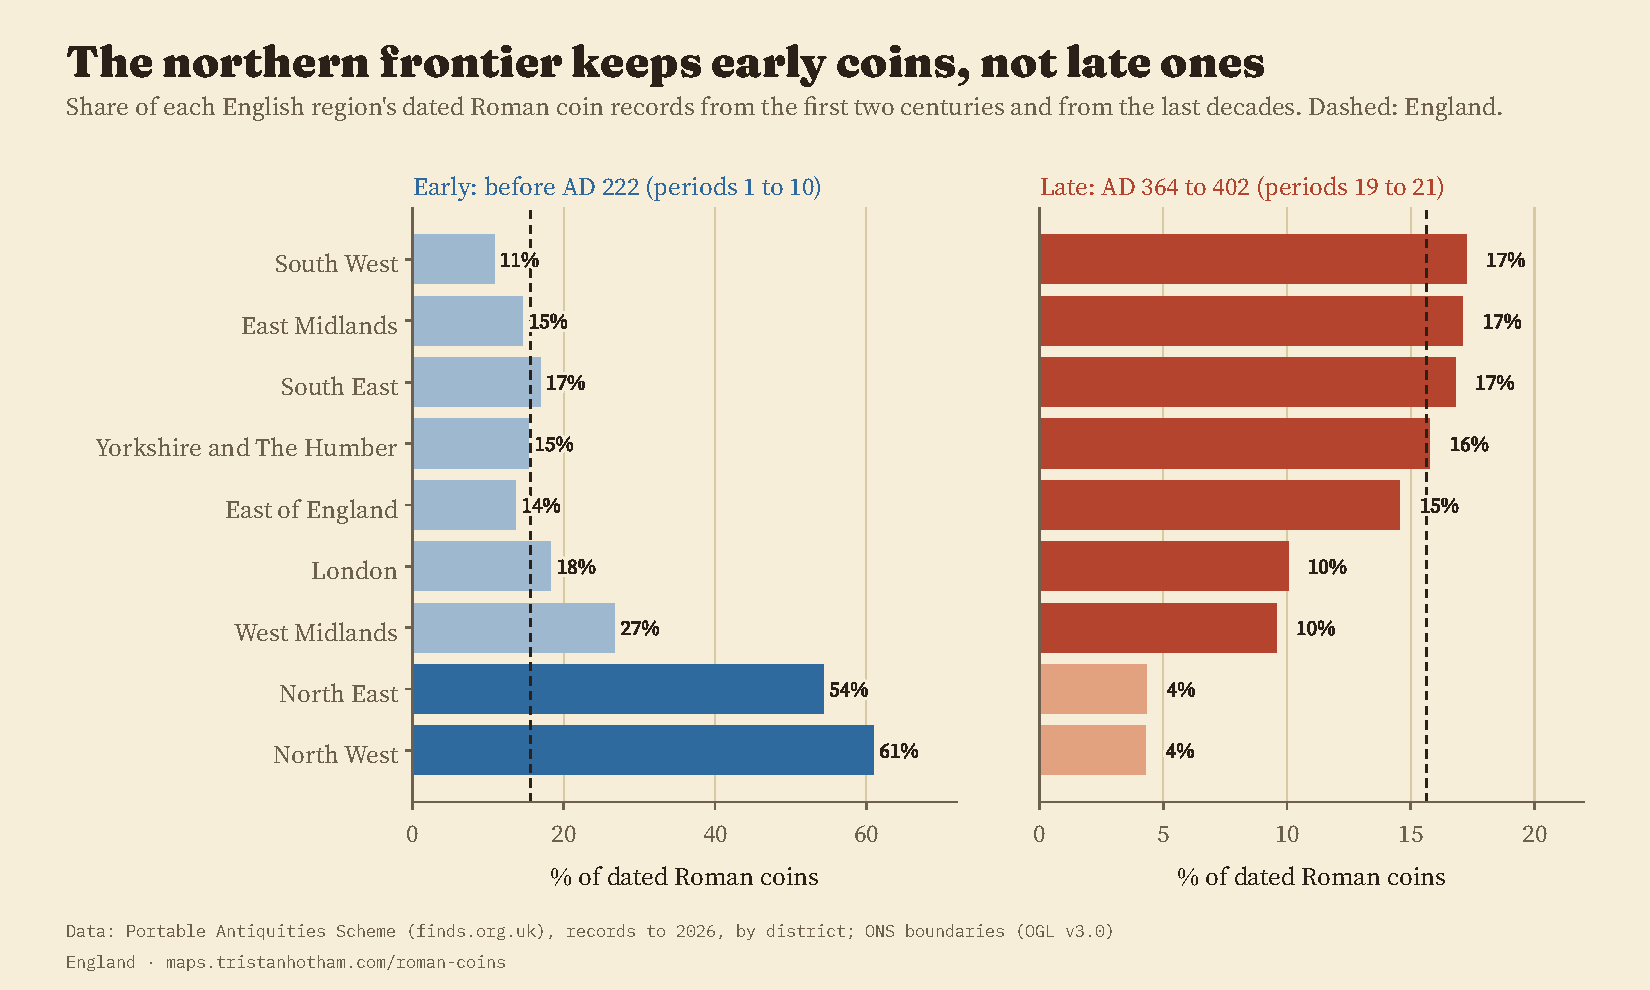
\includegraphics[width=\textwidth]{f_regions.pdf}
\caption{Early (Reece periods 1 to 10, to AD 222) and late (periods 19 to 21, AD 364 to 402) coin records as a share of dated Roman coin records, by English region. Dashed lines: England.}\label{fig:regions}
\end{figure}

A principal component analysis of the per-mille profiles of the 127 districts with at least 100 dated coins tells the same story. The first component explains 0.40 of the variance; periods 1 to 12 load negatively and periods 13, 14 and 16 to 21 positively, so it contrasts early and late coin loss. It correlates at 0.65 with the late share, at 0.33 with easting and at -0.17 with northing: an east to west element is present, but it is weak beside the contrast between the frontier zone and the rest.

Period by period (Figure~\ref{fig:periods} and Figure~\ref{fig:gradients}), the differences are sharper than the grouped shares suggest. The share of coins of AD 193 to 222 rises by a factor of 1.43 per 100 km north (95\% CI 1.21 to 1.69), as does that of AD 222 to 238 (1.40), consistent with the Severan concentration of military activity in the north. Coins of AD 275 to 296, the period that includes the British emperors Carausius and Allectus, rise by 1.31 per 100 km east (1.20 to 1.43), and the last period, AD 388 to 402, by 1.19 per 100 km east (1.06 to 1.35) and by 0.92 per 100 km north. The alternative late definition in the planned checks, periods 20 and 21 only, shows the same eastward lean (1.15, 1.03 to 1.29). So the very latest coins do tilt east, even though the late share as planned (dominated by the abundant Valentinianic issues of period 19) does not. Twenty-one periods tested twice each will produce some intervals that exclude 1 by chance, so these estimates are descriptive.

\begin{figure}[tbp]\centering
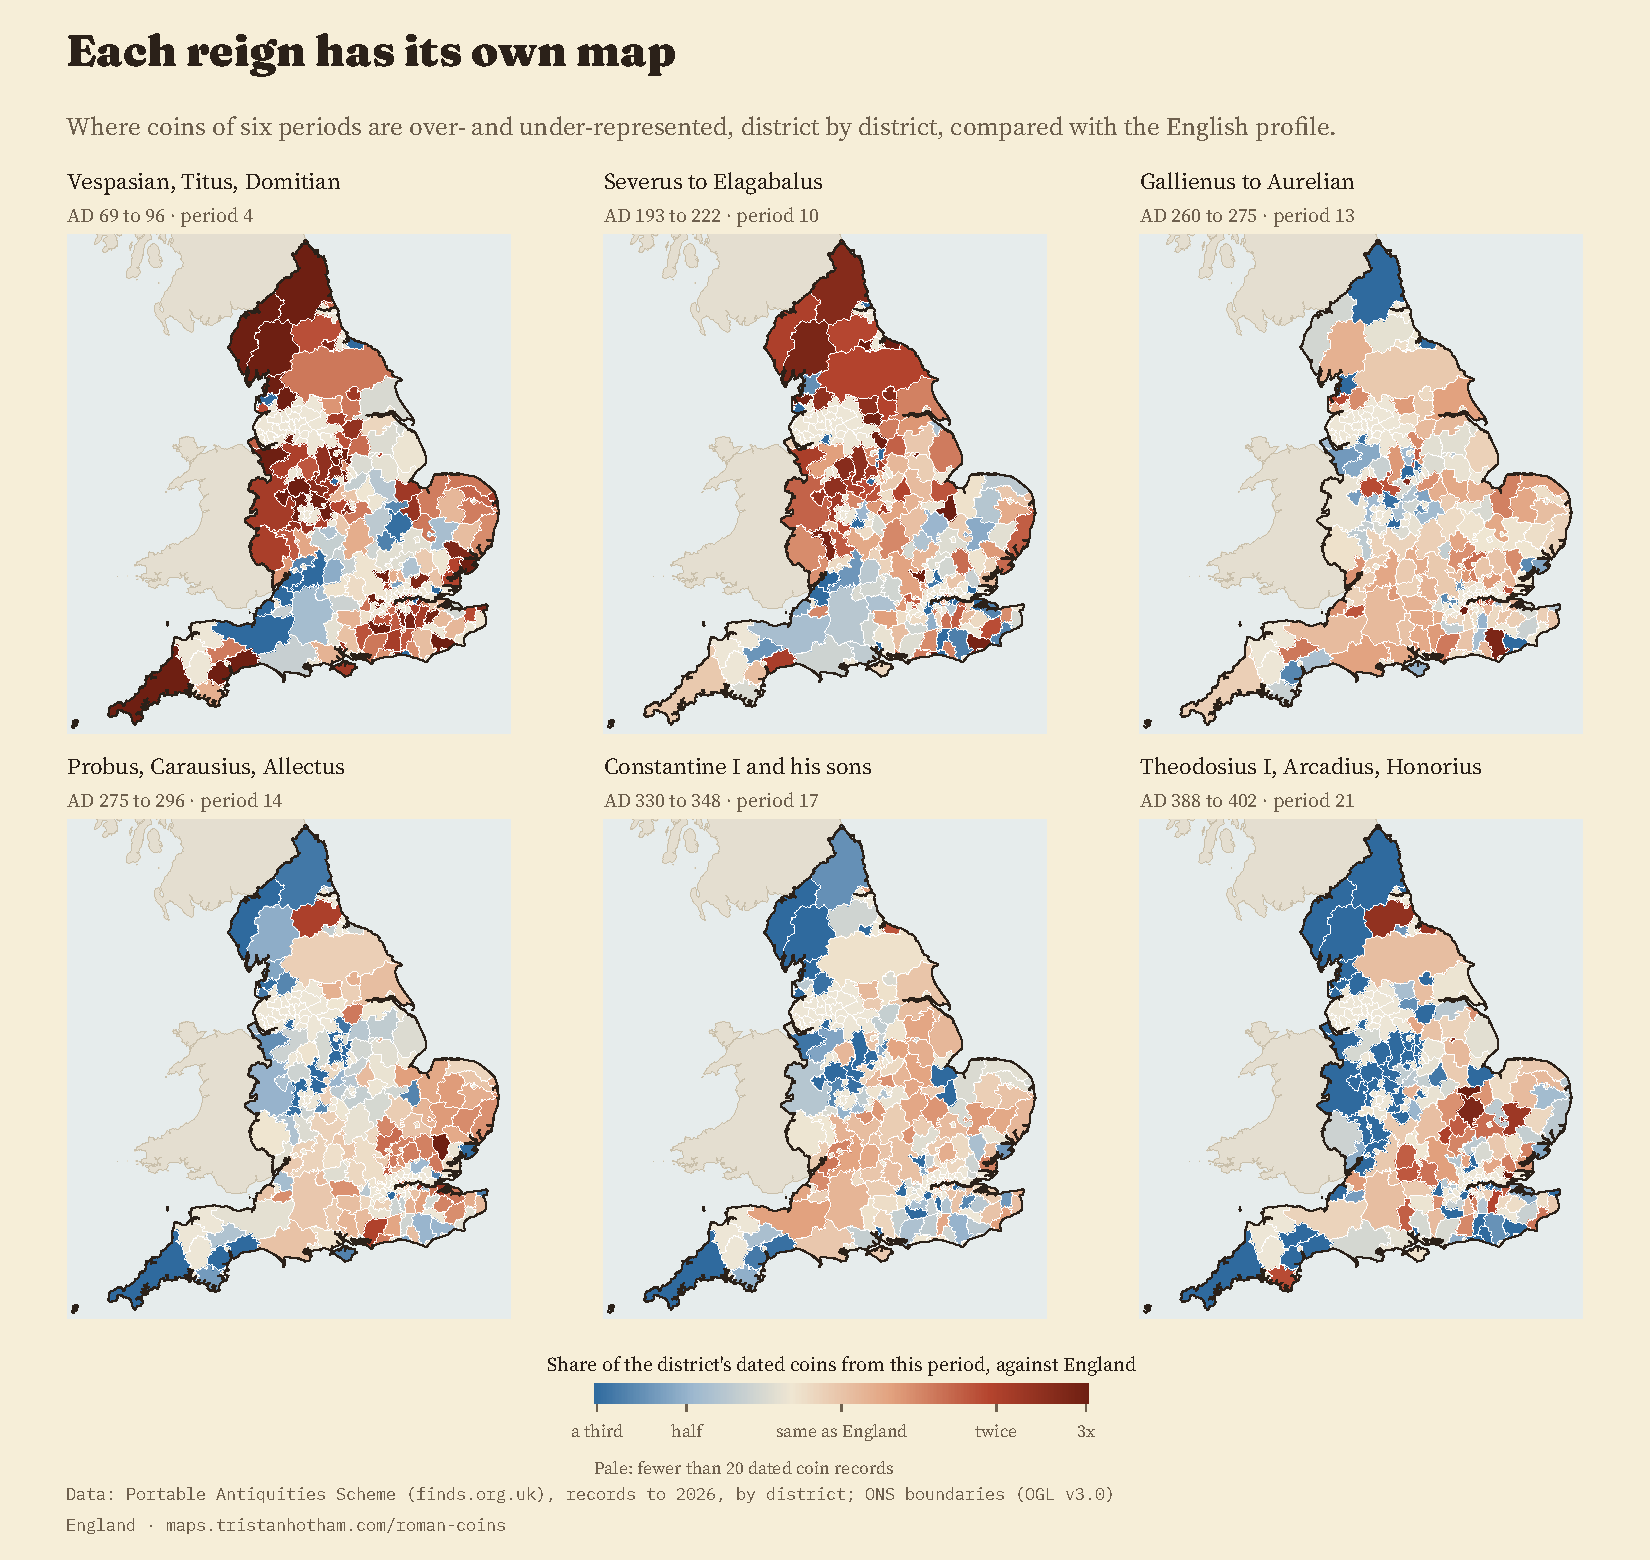
\includegraphics[width=\textwidth]{f_periods.pdf}
\caption{Share of each district's dated coin records from six Reece periods, against England's share for the period ($\log_2$ ratio, capped at a third and three times). Districts with fewer than 20 dated coin records are pale.}\label{fig:periods}
\end{figure}

\begin{figure}[tbp]\centering
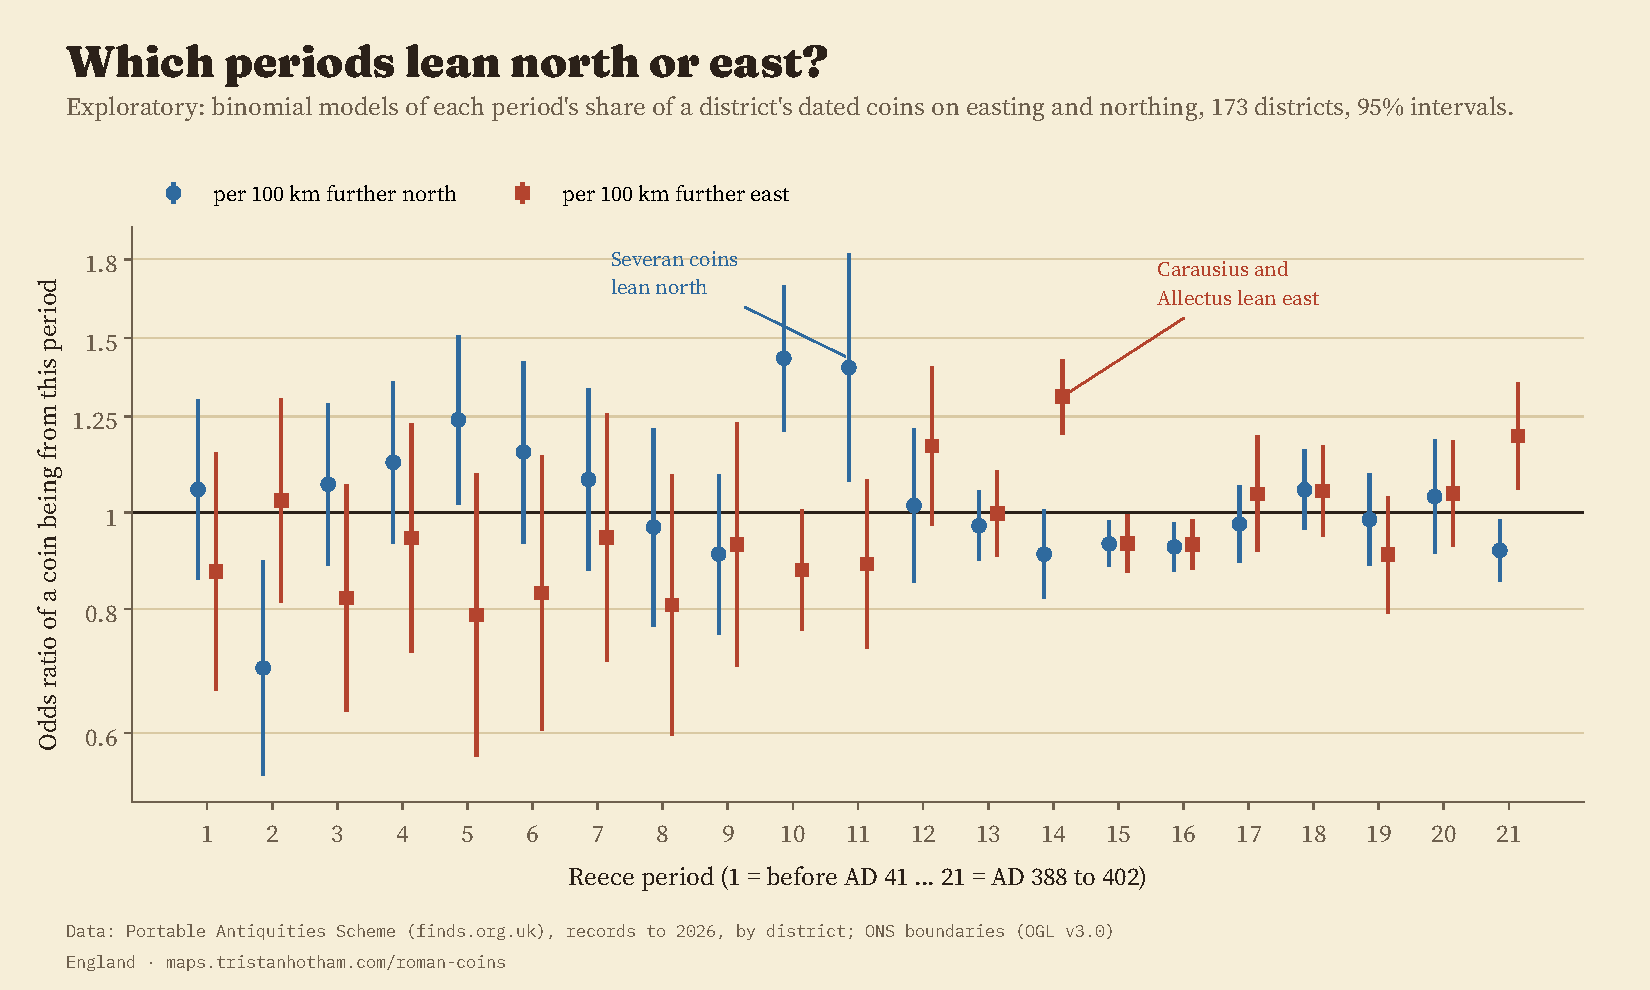
\includegraphics[width=\textwidth]{f_gradients.pdf}
\caption{Exploratory: odds ratios per 100 km north and east for the share of each Reece period in a district's dated coin records, binomial models with standard errors clustered by county, 173 districts, 95\% intervals.}\label{fig:gradients}
\end{figure}

\subsection{Roman coins among all finds}
In England, 259 of every 1,000 PAS records are Roman coins. Figure~\ref{fig:map} maps the district values. Among the 160 districts with at least 500 records, the median is 198 and the interquartile range 112 to 313. The highest values are in Huntingdonshire (605), Hertsmere (558) and West Berkshire (487); the region with the highest value is the South West (328), and the lowest are London (91) and the North West (112). The rank correlation between a district's number of coin records and its coin share is 0.80: districts that produce many Roman coins are also, mostly, districts where Roman coins are a large share of what is found, so the raw counts are not purely an artefact of detecting effort.

\begin{figure}[tbp]\centering
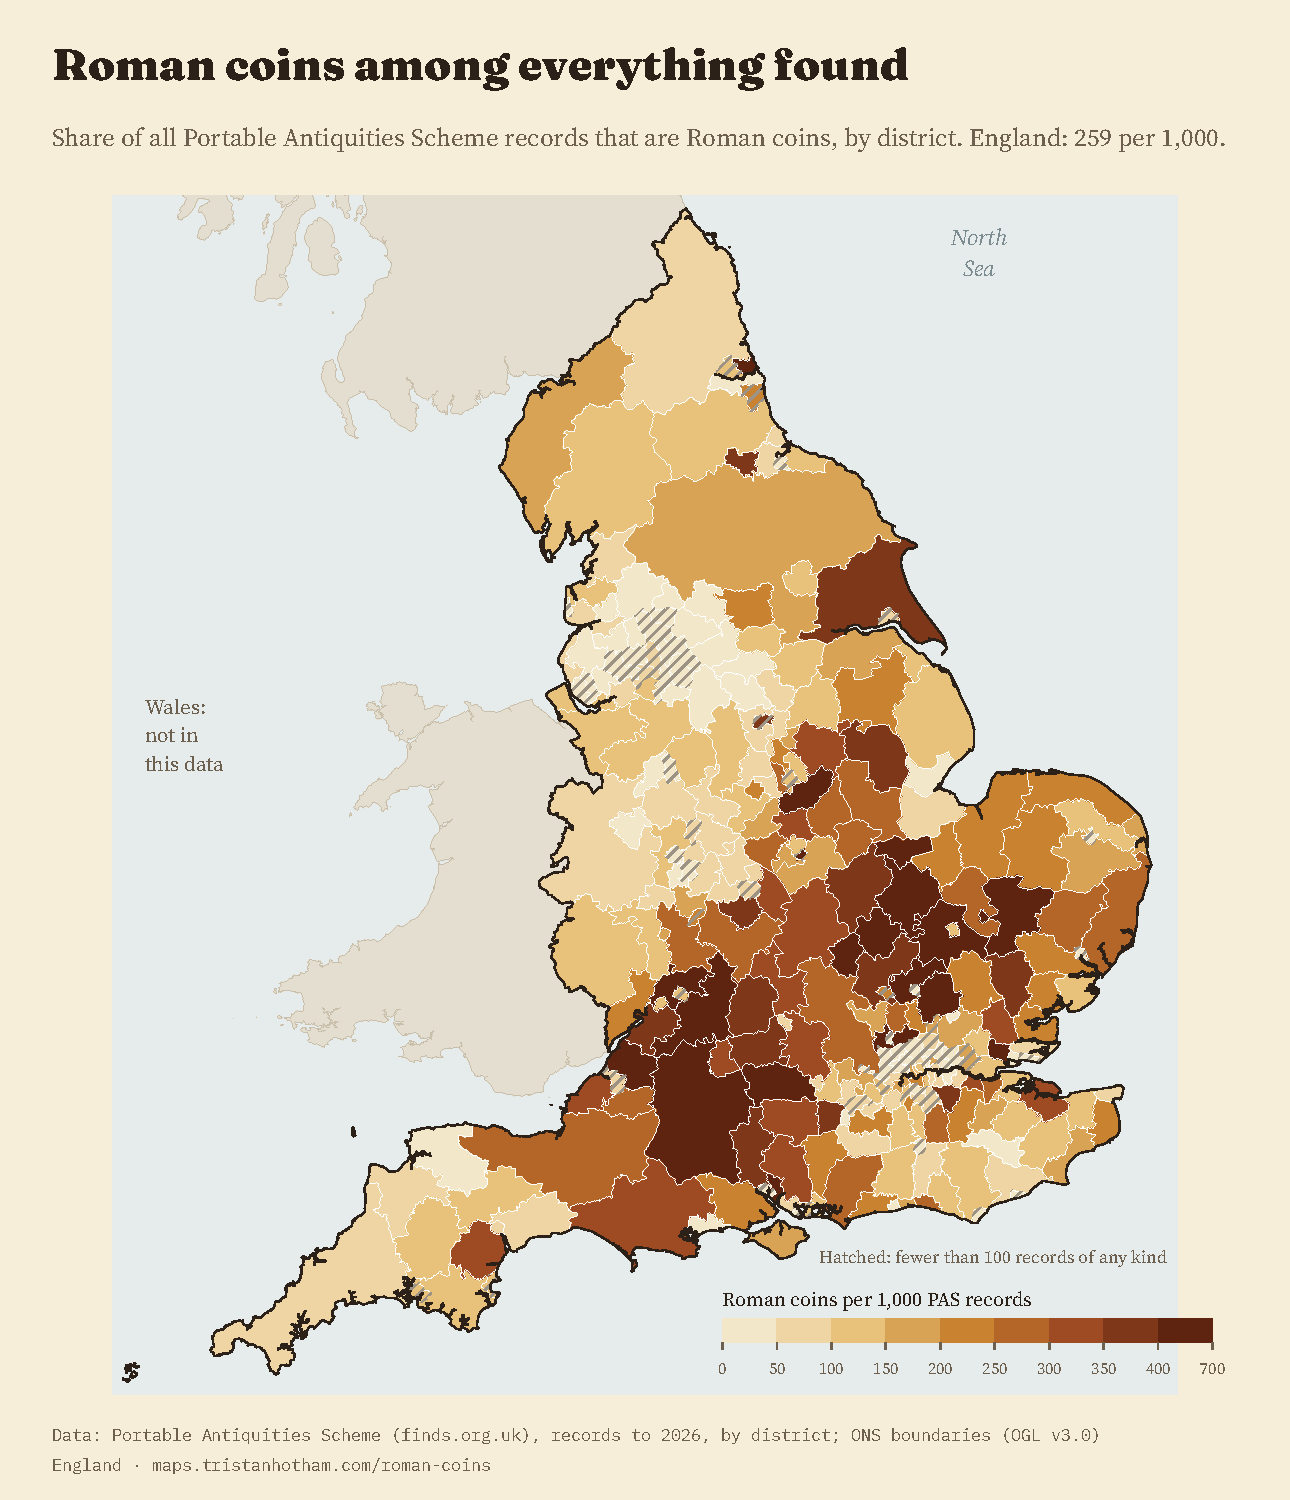
\includegraphics[width=0.78\textwidth]{f_map.pdf}
\caption{Roman coin records per 1,000 PAS records of any period, by English district (ONS 2023). Hatched: fewer than 100 records.}\label{fig:map}
\end{figure}

\subsection{Rulers}
The ruler facets add a descriptive layer (Figure~\ref{fig:rulers}). Nationally, the commonest entry is the House of Constantine without a named ruler (52,374 records), then Constantine I (20,823); local copies of radiate coins of the later third century, the so-called barbarous radiates, are fifth (11,669). Constantine I is the commonest named ruler in 36 of the 47 counties. The exceptions are mostly in the north and west: Trajan in Cumbria, Cheshire, Shropshire and Lancashire, Severus Alexander in Durham, Antoninus Pius in Northumberland and Hadrian in Cornwall and Derbyshire. Constantius II leads in West Yorkshire, and in Staffordshire and Greater Manchester coins of the Roman Republic outnumber those of any single emperor. The county ruler lists are capped at 50 entries, which does not affect the top entry.

\begin{figure}[tbp]\centering
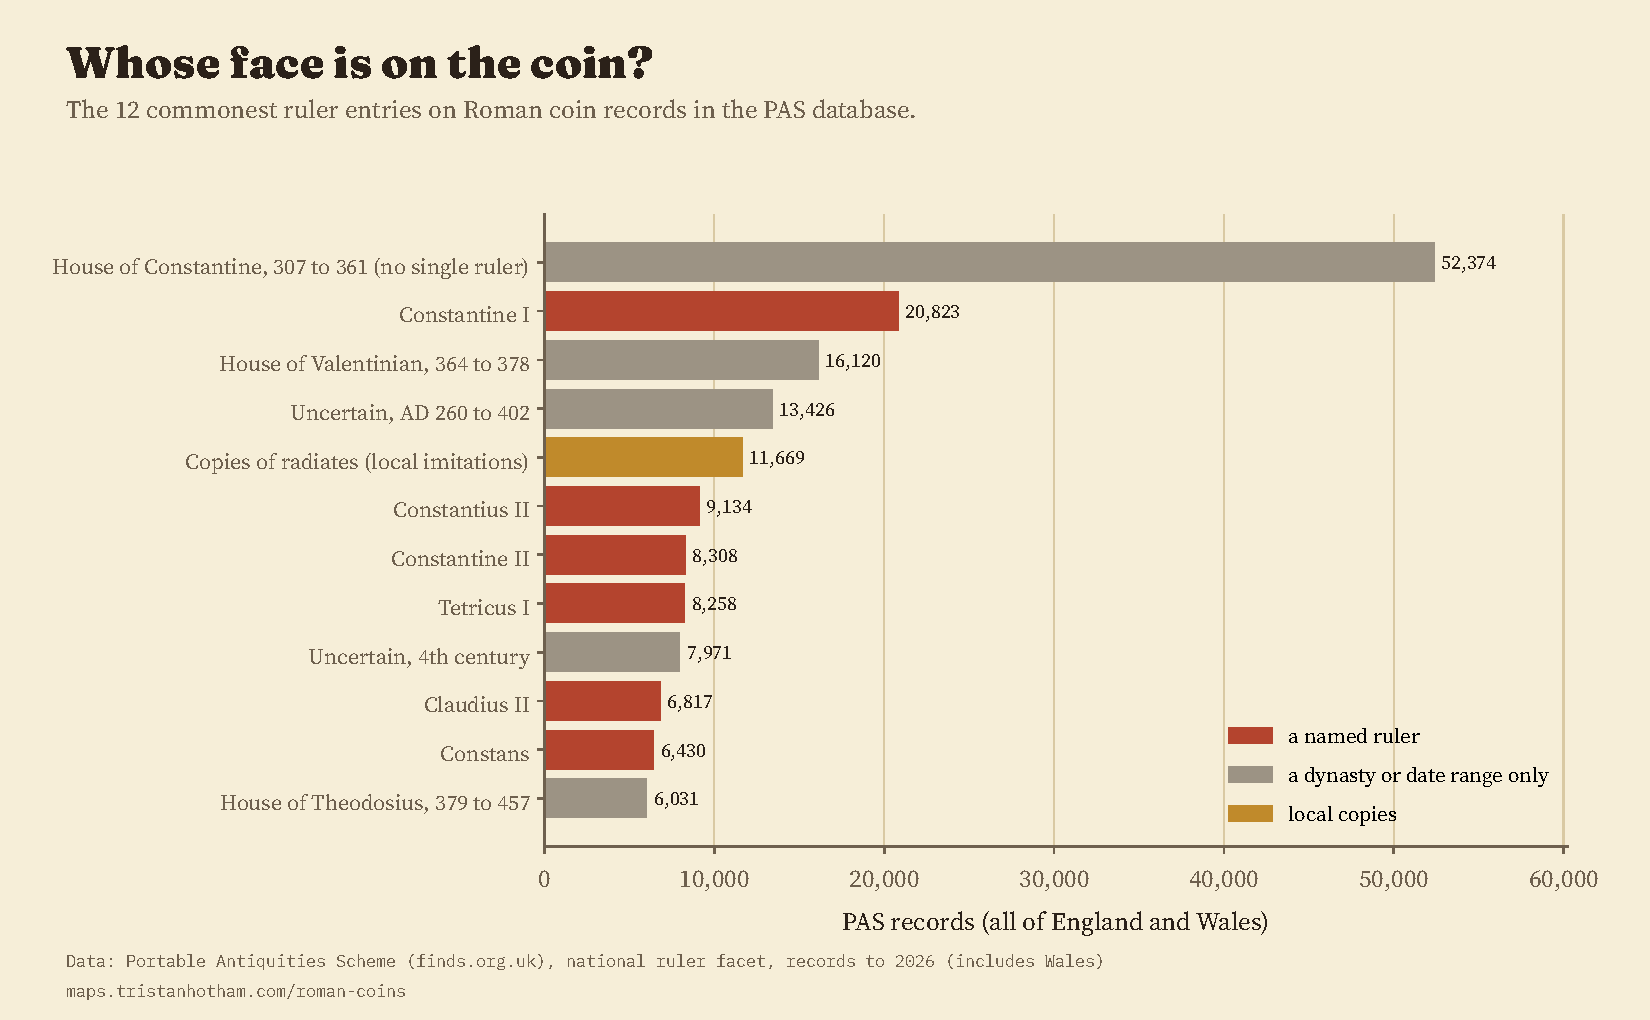
\includegraphics[width=0.95\textwidth]{f_rulers.pdf}
\caption{The 12 commonest ruler entries on Roman coin records in the PAS database (national facet, England and Wales).}\label{fig:rulers}
\end{figure}

\section{Robustness}\label{sec:robust}
Table~\ref{tab:robust} and Figure~\ref{fig:robust} report every planned check for H2 and H3. The null result for the late share does not depend on the threshold of dated coins, the estimator, the level of clustering, any one region, the largest or the most hoard-like districts, or a control for detecting intensity. Across all checks, including leaving out each region, the easting odds ratio for the late share ranges from 0.85 to 1.15 and the northing odds ratio from 0.90 to 1.00. For the early share the northing odds ratio ranges from 1.07 to 1.33: it is above 1 in every check, but its interval includes 1 in most of them, including the main model. Among the checks in Table~\ref{tab:robust}, two give intervals that exclude 1. Defining late as after AD 378 gives an easting odds ratio above 1, as noted above, and the negative binomial count model gives an easting odds ratio below 1 for the early share (0.83, 0.72 to 0.95). In the leave-one-region-out fits (Table~\ref{tab:loro}), leaving out the South East gives a northing ratio of 1.33 (1.05 to 1.68) for the early share and of 0.81 (0.67 to 0.97) for the coin share. These do not change the overall verdict: the planned gradients are weak or absent, and where they appear they depend on the specification. For the coin share (H4) the northing odds ratio is below 1 in every check (range 0.81 to 0.92) but the main interval includes 1.

\begin{figure}[tbp]\centering
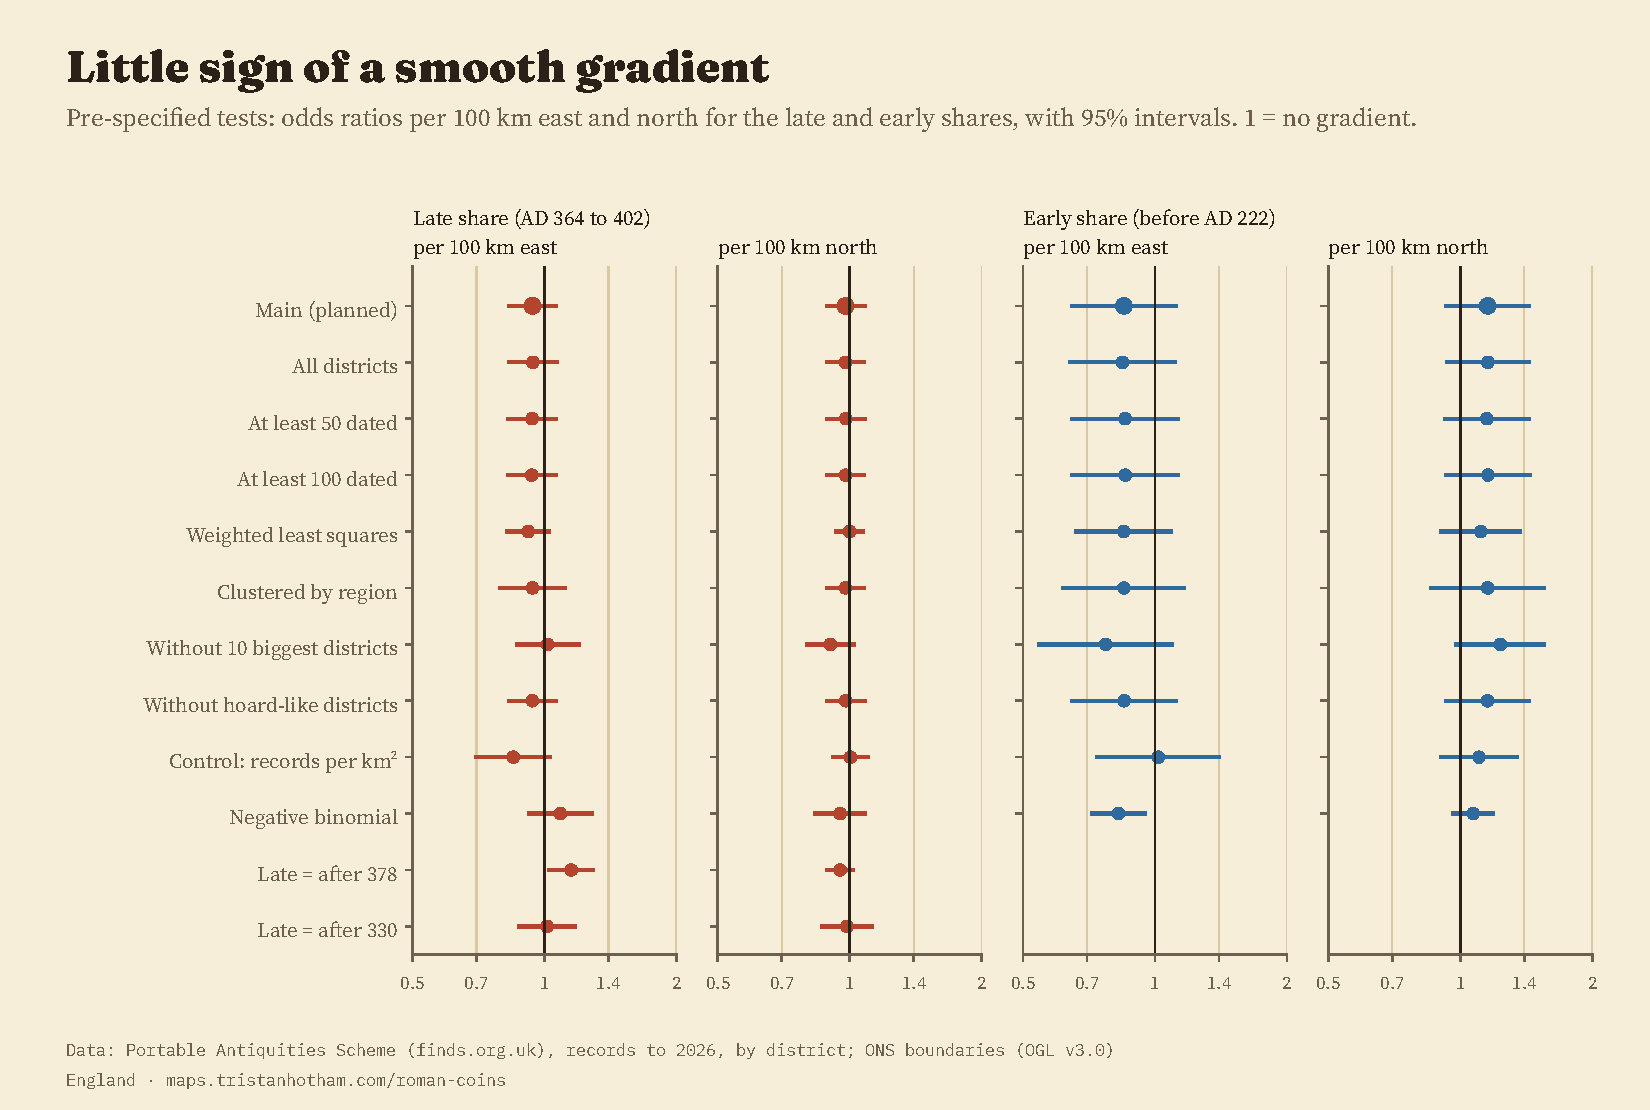
\includegraphics[width=\textwidth]{f_robust.pdf}
\caption{Planned tests of H2 (late share) and H3 (early share) under each robustness check: odds ratios per 100 km east and north with 95\% confidence intervals.}\label{fig:robust}
\end{figure}

\begin{table}[tbp]\centering\scriptsize\caption{Robustness of the planned tests: odds ratios per 100 km [95\% CI]. The leave-one-region-out fits are in Table~\ref{tab:loro}.}\label{tab:robust}\begin{tabular}{lrrrrr}\toprule & \multicolumn{2}{c}{H2: late share} & \multicolumn{2}{c}{H3: early share} & \\ Check & East & North & East & North & N\\\midrule
Main (planned) & 0.94 [0.83, 1.06] & 0.98 [0.89, 1.08] & 0.85 [0.65, 1.12] & 1.16 [0.93, 1.43] & 173\\
All districts with a dated coin & 0.94 [0.83, 1.06] & 0.98 [0.89, 1.08] & 0.84 [0.64, 1.11] & 1.16 [0.93, 1.43] & 270\\
At least 50 dated & 0.94 [0.83, 1.06] & 0.98 [0.89, 1.08] & 0.85 [0.65, 1.13] & 1.15 [0.92, 1.43] & 149\\
At least 100 dated & 0.94 [0.82, 1.06] & 0.98 [0.89, 1.08] & 0.86 [0.65, 1.13] & 1.16 [0.93, 1.44] & 127\\
WLS, empirical logit & 0.92 [0.82, 1.02] & 1.00 [0.93, 1.07] & 0.85 [0.66, 1.09] & 1.11 [0.91, 1.37] & 173\\
Clustered by region & 0.94 [0.79, 1.12] & 0.98 [0.89, 1.08] & 0.85 [0.62, 1.17] & 1.16 [0.86, 1.55] & 173\\
Without 10 largest districts & 1.02 [0.86, 1.19] & 0.90 [0.80, 1.02] & 0.77 [0.55, 1.09] & 1.23 [0.98, 1.55] & 163\\
Without hoard-like districts & 0.94 [0.83, 1.06] & 0.98 [0.89, 1.08] & 0.85 [0.65, 1.12] & 1.15 [0.93, 1.43] & 169\\
Control: log records per km$^2$ & 0.85 [0.70, 1.03] & 1.00 [0.92, 1.10] & 1.02 [0.74, 1.40] & 1.10 [0.90, 1.35] & 173\\
Negative binomial & 1.09 [0.92, 1.28] & 0.95 [0.83, 1.08] & 0.83 [0.72, 0.95] & 1.07 [0.96, 1.19] & 173\\
Late = AD 378 to 402 & 1.15 [1.03, 1.29] & 0.95 [0.89, 1.02] &  &  & 173\\
Late = AD 330 to 402 & 1.01 [0.88, 1.17] & 0.99 [0.86, 1.12] &  &  & 173\\
\midrule
Permutation $p$, H2 & \multicolumn{4}{l}{east 0.351, north 0.686 (999 shuffles)} & \\
Permutation $p$, H3 & \multicolumn{4}{l}{east 0.147, north 0.079 (999 shuffles)} & \\
\bottomrule\end{tabular}\end{table}

\section{Discussion}\label{sec:disc}
\subsection{What the pattern says}
The PAS has made it possible to describe coin loss over the whole of England, district by district, from records that anyone can query. The English profile is the British site-find profile: the third-century radiate surge, the Constantinian peak, the Valentinianic high and the sharp fall after AD 378. That a dataset built from finds in ploughsoil reproduces a curve first drawn from excavated towns, forts and villas is itself a confirmation of the method's central assumption, that site finds sample the coins in circulation in a broadly similar way wherever they are found \citep{reece1995,walton2012}.

The planned regional tests are less comfortable. A smooth tilt towards the south and east in late coin loss, and towards the north and west in early coin loss, is a natural way to formalise the contrast between the civil and military zones of the province, and it is not what the data show. The late share is no higher in the east than in the west: the South West, with the villa landscapes of Somerset, Gloucestershire and Wiltshire, has the highest late share of any region, and the east coast is not especially late. This agrees with Henry's parish maps, in which the strongest late fourth-century loss lies in a band from Hampshire and Wiltshire to the East Midlands, with coastal areas of the east in the lower quartile \citep{henry2024}. What the data show instead is a step at the edge of the frontier zone. In the North East and North West the profile is dominated by first- and second-century coins and the late fourth century is almost absent; elsewhere, including Yorkshire and the Humber, the profile looks broadly like the English mean. The contrast is consistent with the distributions of late silver mapped by \citet{walton2016}, rare in the north-west and north-east and extending north only into parts of Yorkshire, and with Henry's finding that ever fewer military sites fall in the upper quartile of coin loss in the later fourth century \citep{henry2024}. One reading is that early coin loss in the north reflects the army, and late coin loss a monetised rural economy that the frontier zone shared less; the data here cannot separate that reading from differences in recovery.

The period-by-period results add detail. The Severan periods lean north, as the military history of the early third century would suggest, and the coins of AD 275 to 296 lean east. The latest coins of all, AD 388 to 402, lean east and south even though the late share as a whole does not. These patterns were not tested in advance and include many comparisons, so they should be checked against independent data, such as the excavated assemblages in Henry's corpus, before they are relied on.

\subsection{Relation to earlier work}
The results sit between two earlier bodies of work. Reece's British mean was drawn from excavated sites, mostly towns, forts and villas \citep{reece1991,reece1995}. The PAS profile is drawn mostly from ploughsoil on rural land, much of it away from known sites \citep{brindle2014}. That the two curves share their peaks and troughs suggests that the rhythm of supply, rather than the type of site, sets the broad shape of coin loss in the province, as Reece argued. \citet{walton2016} note one difference in the detail: late silver siliquae are proportionally more common in the PAS rural data than on urban sites.

The regional result is closest to \citet{henry2024}, who mapped quartiles of per-mille values for 1,421 parishes. Henry's maps show the strongest late fourth-century loss in a band through Hampshire, Wiltshire, Gloucestershire, Oxfordshire and the East Midlands, with coastal parishes of the east in the lower quartile. That band runs from south west to north east, and a gradient fitted on easting and northing would largely miss it. The present analysis adds three things to Henry's: a formal test of the simplest gradient hypothesis, with a pre-specified plan and a clear null; a denominator for recording intensity built from all PAS records, which a corpus of coins alone cannot provide; and a district-level table that can be refreshed directly from the public search. It also loses things that Henry's corpus has: the excavated assemblages, the parish scale and site types.

The use of all finds as a denominator follows the logic of \citet{bevan2012}, who argued that artefact distributions should be judged against the distribution of all recorded finds. It is a partial answer to the biases set out by \citet{robbins2012,robbins2013}. It removes the effect of how much detecting and recording happens in a district, but not of what is selected within that total. A district where detectorists favour Roman sites, or where Finds Liaison Officers record Roman coins more fully than post-medieval buttons, will have a high coin share for reasons that have nothing to do with the Roman past. The rank correlation of 0.80 between raw coin counts and coin shares shows that the two measures largely agree, which is reassuring but not decisive.

\subsection{Limitations}
Five limits matter. First, the PAS records what is found and reported, and the denominator corrects only for the overall volume of recording. Differences in land use, in the visibility of small late bronze coins, and in what detectorists choose to show to Finds Liaison Officers can still shape the profiles \citep{robbins2012,robbins2013}. Second, counts are records, not coins, and hoards recorded coin by coin can dominate a district; the checks that drop large and concentrated districts reduce, but cannot remove, this effect, because the facet counts do not distinguish hoard records. Third, districts are coarse and uneven units; a gradient between districts says nothing about patterns within them, and the step at the northern regions could be partly a boundary drawn by the analyst. Fourth, Wales is missing, so the western half of the military zone is not observed. Fifth, the design is descriptive: it shows where coins of each period were lost and recorded, not why.

\subsection{Implications}
For coin specialists, the result suggests that regional comparisons with the British mean should allow for a frontier zone that behaves differently from everywhere else, rather than assuming a gradient across the lowland. For users of the PAS, the paper shows that the public facet counts, with the all-finds denominator, are enough to reproduce the main features of the British coin curve and to test regional hypotheses at national scale, in a form that can be refreshed every year as new records are added. And for the debate about the end of Roman Britain, the eastward lean of the very last coins is a pattern worth testing in the excavated record.

\section{Conclusion}\label{sec:conc}
Using 275,206 Roman coin records from the Portable Antiquities Scheme, set against 1,062,032 records of all periods, this paper has shown that the English profile of Roman coin loss reproduces Reece's British curve, that the pre-specified expectation of smooth regional gradients in early and late coin loss is not supported, and that regional variation takes the form of a sharp contrast between the northern frontier regions and the rest of England. The null result is not a failure of the data: it is a reminder that the simplest map of Roman Britain, a tilt from a civil south east to a military north west, does not describe how coins were lost across the English countryside.

\section*{Data availability statement}
Data and code: Zenodo DOI https://doi.org/10.5281/zenodo.24115196. The archive contains the district table (all records, Roman coin records and records by Reece period for each of 296 English districts), the national and county tables, the county ruler lists, the analysis plan, every estimate and all code. The underlying records are those of the Portable Antiquities Scheme (\url{https://finds.org.uk}); only aggregate counts are republished. With thanks to the finders and recorders.

\section*{AI statement}
I wrote the text, with drafting and editing assistance from Claude (Anthropic), which also helped prepare the analysis code. I reviewed and checked all text and results.

\begin{thebibliography}{99}
\bibitem[Allen et al.(2017)]{allen2017} Allen, M., Lodwick, L., Brindle, T., Fulford, M. and Smith, A. (2017) \textit{The Rural Economy of Roman Britain. New Visions of the Countryside of Roman Britain, Volume 2}. Britannia Monograph 30. London: Society for the Promotion of Roman Studies.
\bibitem[Bevan(2012)]{bevan2012} Bevan, A. (2012) Spatial methods for analysing large-scale artefact inventories. \textit{Antiquity} 86(332), 492 to 506.
\bibitem[Bland(2005)]{bland2005} Bland, R. (2005) A pragmatic approach to the problem of portable antiquities: the experience of England and Wales. \textit{Antiquity} 79(304), 440 to 447. doi:10.1017/S0003598X00114218.
\bibitem[Bland(2018)]{bland2018} Bland, R. (2018) \textit{Coin Hoards and Hoarding in Roman Britain AD 43 to c. 498}. British Numismatic Society Special Publication 13. London: Spink.
\bibitem[Bland et al.(2017)]{bland2017} Bland, R., Lewis, M., Pett, D., Richardson, I., Robbins, K. and Webley, R. (2017) The Treasure Act and Portable Antiquities Scheme in England and Wales. In G. Moshenska (ed.), \textit{Key Concepts in Public Archaeology}, 107 to 121. London: UCL Press. doi:10.14324/111.9781911576419.
\bibitem[Brindle(2013)]{brindle2013} Brindle, T. (2013) Making the most of PAS data: macro- and micro-level studies of Romano-British settlement. \textit{Landscapes} 14(1), 73 to 91.
\bibitem[Brindle(2014)]{brindle2014} Brindle, T. (2014) \textit{The Portable Antiquities Scheme and Roman Britain}. British Museum Research Publication 196. London: British Museum.
\bibitem[Brindle(2017)]{brindle2017} Brindle, T. (2017) Coins and markets in the countryside. In \citet{allen2017}, 237 to 277.
\bibitem[Cameron and Miller(2015)]{cameron2015} Cameron, A. C. and Miller, D. L. (2015) A practitioner's guide to cluster-robust inference. \textit{Journal of Human Resources} 50(2), 317 to 372.
\bibitem[Casey(1986)]{casey1986} Casey, P. J. (1986) \textit{Understanding Ancient Coins: An Introduction for Archaeologists and Historians}. London: Batsford.
\bibitem[Collins(2012)]{collins2012} Collins, R. (2012) \textit{Hadrian's Wall and the End of Empire: The Roman Frontier in the 4th and 5th Centuries}. New York and Abingdon: Routledge.
\bibitem[Cooper and Green(2016)]{cooper2016} Cooper, A. and Green, C. (2016) Embracing the complexities of ``big data'' in archaeology: the case of the English Landscape and Identities project. \textit{Journal of Archaeological Method and Theory} 23, 271 to 304. doi:10.1007/s10816-015-9240-4.
\bibitem[Davies and Gregory(1991)]{davies1991} Davies, J. A. and Gregory, T. (1991) Coinage from a civitas: a survey of the Roman coins found in Norfolk and their contribution to the archaeology of the Civitas Icenorum. \textit{Britannia} 22, 65 to 101. doi:10.2307/526631.
\bibitem[Esmonde Cleary(1989)]{esmondecleary1989} Esmonde Cleary, A. S. (1989) \textit{The Ending of Roman Britain}. London: Batsford.
\bibitem[Fox(1932)]{fox1932} Fox, C. (1932) \textit{The Personality of Britain: Its Influence on Inhabitant and Invader in Prehistoric and Early Historic Times}. Cardiff: National Museum of Wales.
\bibitem[Gerrard(2013)]{gerrard2013} Gerrard, J. (2013) \textit{The Ruin of Roman Britain: An Archaeological Perspective}. Cambridge: Cambridge University Press.
\bibitem[Henry(2024)]{henry2024} Henry, R. (2024) A new corpus of Roman coins from England and Wales: an overview of the evidence and analysis of the data. \textit{Britannia} 55, 47 to 81. doi:10.1017/S0068113X2400028X.
\bibitem[Kemmers and Myrberg(2011)]{kemmers2011} Kemmers, F. and Myrberg, N. (2011) Rethinking numismatics: the archaeology of coins. \textit{Archaeological Dialogues} 18(1), 87 to 108. doi:10.1017/S1380203811000146.
\bibitem[Lewis(2016)]{lewis2016} Lewis, M. (2016) A detectorist's utopia? Archaeology and metal-detecting in England and Wales. \textit{Open Archaeology} 2(1). doi:10.1515/opar-2016-0009.
\bibitem[Lockyear(2000)]{lockyear2000} Lockyear, K. (2000) Site finds in Roman Britain: a comparison of techniques. \textit{Oxford Journal of Archaeology} 19(4), 397 to 423.
\bibitem[Mattingly(2006)]{mattingly2006} Mattingly, D. (2006) \textit{An Imperial Possession: Britain in the Roman Empire, 54 BC to AD 409}. London: Allen Lane.
\bibitem[Millett(1990)]{millett1990} Millett, M. (1990) \textit{The Romanization of Britain: An Essay in Archaeological Interpretation}. Cambridge: Cambridge University Press.
\bibitem[Moorhead(2013)]{moorhead2013} Moorhead, S. (2013) \textit{A History of Roman Coinage in Britain, Illustrated by Finds Recorded with the Portable Antiquities Scheme}. Greenlight Publishing.
\bibitem[Moorhead and Walton(2014)]{moorhead2014} Moorhead, S. and Walton, P. (2014) Coinage at the end of Roman Britain. In F. K. Haarer (ed.), \textit{AD 410: The History and Archaeology of Late and Post-Roman Britain}, 99 to 116. London: Society for the Promotion of Roman Studies.
\bibitem[Nomisma.org(2026)]{nomisma} Nomisma.org (2026) Reece periods 1 to 24 (\texttt{reece1} to \texttt{reece24}). CC BY. \url{https://github.com/nomisma/data}. Retrieved 2026.
\bibitem[ONS(2023)]{ons2023} Office for National Statistics (2023) \textit{Local Authority Districts (December 2023) Boundaries UK BSC}. ONS Open Geography Portal. Open Government Licence v3.0.
\bibitem[Papke and Wooldridge(1996)]{papke1996} Papke, L. E. and Wooldridge, J. M. (1996) Econometric methods for fractional response variables with an application to 401(k) plan participation rates. \textit{Journal of Applied Econometrics} 11(6), 619 to 632.
\bibitem[PAS(2026)]{pas2026} Portable Antiquities Scheme (2026) \textit{PAS database}, \url{https://finds.org.uk}. British Museum and Amgueddfa Cymru. Facet counts retrieved 2026.
\bibitem[Reece(1972)]{reece1972} Reece, R. (1972) A short survey of the Roman coins found on fourteen sites in Britain. \textit{Britannia} 3, 269 to 276. doi:10.2307/526030.
\bibitem[Reece(1987)]{reece1987} Reece, R. (1987) \textit{Coinage in Roman Britain}. London: Seaby.
\bibitem[Reece(1991)]{reece1991} Reece, R. (1991) \textit{Roman Coins from 140 Sites in Britain}. Cotswold Studies 4. Cirencester.
\bibitem[Reece(1995)]{reece1995} Reece, R. (1995) Site-finds in Roman Britain. \textit{Britannia} 26, 179 to 206. doi:10.2307/526876.
\bibitem[Richards et al.(2009)]{richards2009} Richards, J. D., Naylor, J. and Holas-Clark, C. (2009) Anglo-Saxon landscape and economy: using portable antiquities to study Anglo-Saxon and Viking Age England. \textit{Internet Archaeology} 25.
\bibitem[Robbins(2012)]{robbins2012} Robbins, K. (2012) \textit{From Past to Present: Understanding the Impact of Sampling Bias on Data Recorded by the Portable Antiquities Scheme}. PhD thesis, University of Southampton.
\bibitem[Robbins(2013)]{robbins2013} Robbins, K. (2013) Balancing the scales: exploring the variable effects of collection bias on data collected by the Portable Antiquities Scheme. \textit{Landscapes} 14(1), 54 to 72. doi:10.1179/1466203513Z.0000000006.
\bibitem[Ryan(1988)]{ryan1988} Ryan, N. S. (1988) \textit{Fourth-Century Coin Finds from Roman Britain: A Computer Analysis}. BAR British Series 183. Oxford: BAR.
\bibitem[Seabold and Perktold(2010)]{seabold2010} Seabold, S. and Perktold, J. (2010) statsmodels: econometric and statistical modeling with Python. \textit{Proceedings of the 9th Python in Science Conference}, 92 to 96.
\bibitem[Smith et al.(2016)]{smith2016} Smith, A., Allen, M., Brindle, T. and Fulford, M. (2016) \textit{The Rural Settlement of Roman Britain. New Visions of the Countryside of Roman Britain, Volume 1}. Britannia Monograph 29. London: Society for the Promotion of Roman Studies.
\bibitem[Walton(2012)]{walton2012} Walton, P. (2012) \textit{Rethinking Roman Britain: Coinage and Archaeology}. Collection Moneta 137. Wetteren: Moneta.
\bibitem[Walton and Moorhead(2016)]{walton2016} Walton, P. and Moorhead, S. (2016) Coinage and collapse? The contribution of numismatic data to understanding the end of Roman Britain. \textit{Internet Archaeology} 41. doi:10.11141/ia.41.8.
\end{thebibliography}

\appendix
\section{Regional figures and data construction}\label{sec:appx}
Table~\ref{tab:regions} gives the regional totals and shares used in Figure~\ref{fig:regions}. The district table is built as follows. For each ceremonial county, the district facet of all records, of Roman coin records, and of Roman coin records in each Reece period is read and summed by district name across counties. Every district name was matched to the ONS December 2023 list; there were no unmatched names. Districts are assigned to regions by the region polygon containing a point inside the district, using the ONS region boundaries. Coordinates are that point's easting and northing (British National Grid). The rural settlement synthesis of \citet{smith2016} and the economic volume of \citet{allen2017} give the settlement and market context against which the district patterns can be read.

\begin{table}[htbp]\centering\small\caption{English regions: all records, Roman coin records, coins per 1,000 records, dated coin records and early and late shares (\%).}\label{tab:regions}\begin{tabular}{lrrrrrr}\toprule Region & Records & Coins & Per 1,000 & Dated & Early & Late\\\midrule
East Midlands & 160,713 & 41,610 & 259 & 27,604 & 14.6 & 17.1\\
East of England & 296,457 & 85,143 & 287 & 54,280 & 13.6 & 14.6\\
London & 16,054 & 1,466 & 91 & 1,165 & 18.3 & 10.0\\
North East & 11,357 & 2,171 & 191 & 1,775 & 54.3 & 4.3\\
North West & 24,459 & 2,749 & 112 & 2,069 & 60.9 & 4.3\\
South East & 236,106 & 62,152 & 263 & 42,802 & 16.9 & 16.8\\
South West & 130,584 & 42,867 & 328 & 33,595 & 10.8 & 17.2\\
West Midlands & 65,134 & 11,238 & 173 & 6,570 & 26.7 & 9.6\\
Yorkshire and The Humber & 121,168 & 25,810 & 213 & 18,971 & 15.3 & 15.8\\
\bottomrule\end{tabular}\end{table}

\begin{table}[htbp]\centering\scriptsize\caption{Leaving out one region at a time: odds ratios per 100 km [95\% CI].}\label{tab:loro}\begin{tabular}{lrrrrr}\toprule Region left out & H2 east & H2 north & H3 east & H3 north & H4 north\\\midrule
East Midlands & 0.94 [0.83, 1.06] & 0.95 [0.85, 1.06] & 0.86 [0.66, 1.12] & 1.19 [0.95, 1.50] & 0.89 [0.76, 1.05]\\
East of England & 1.07 [0.89, 1.29] & 0.95 [0.86, 1.05] & 0.76 [0.45, 1.29] & 1.17 [0.93, 1.47] & 0.91 [0.79, 1.05]\\
London & 0.94 [0.83, 1.07] & 0.98 [0.88, 1.08] & 0.85 [0.64, 1.11] & 1.16 [0.93, 1.44] & 0.88 [0.77, 1.02]\\
North East & 0.92 [0.82, 1.04] & 1.00 [0.92, 1.10] & 0.89 [0.67, 1.18] & 1.08 [0.88, 1.34] & 0.90 [0.77, 1.04]\\
North West & 0.91 [0.81, 1.03] & 1.00 [0.92, 1.10] & 0.94 [0.72, 1.22] & 1.07 [0.87, 1.32] & 0.91 [0.79, 1.06]\\
South East & 0.98 [0.85, 1.14] & 0.97 [0.85, 1.11] & 0.77 [0.55, 1.06] & 1.33 [1.05, 1.68] & 0.81 [0.67, 0.97]\\
South West & 0.91 [0.77, 1.07] & 0.98 [0.88, 1.09] & 0.73 [0.53, 1.00] & 1.07 [0.87, 1.31] & 0.92 [0.78, 1.07]\\
West Midlands & 0.91 [0.80, 1.03] & 0.99 [0.90, 1.09] & 0.90 [0.67, 1.19] & 1.13 [0.91, 1.42] & 0.91 [0.79, 1.05]\\
Yorkshire and The Humber & 0.94 [0.82, 1.08] & 0.96 [0.82, 1.13] & 0.83 [0.63, 1.10] & 1.26 [0.94, 1.70] & 0.91 [0.79, 1.05]\\
\bottomrule\end{tabular}\end{table}

\end{document}
